\section{Portfolio choice: asset classes, risk aversion and efficient portfolios}

These entries build on \hyperref[meth:portfolio-return-moments]{portfolio return moments} and \hyperref[mech:diversification-correlation]{diversification}. The historical table is dated, single-country evidence. The three-fund example is invented, with one-year expected returns, standard deviations and correlations stated in US dollars; it illustrates mechanics and is not a forecast. Its inputs are $\mu=(8,3.5,6)$ percent and $\sigma=(18,6,12)$ percent for an equity fund E, a bond fund B and a property fund P, with correlations $\rho_{EB}=0.1$, $\rho_{EP}=0.6$ and $\rho_{BP}=0.3$, and a risk-free rate of 3 percent where one is used.

\begin{qfdefinition}[Asset classes and their characteristics: cash, government and corporate bonds, equities, real estate and gold; risk, return, income, liquidity and inflation exposure; dated historical returns against expected returns]\label{def:asset-class-characteristics}
\qffield{Statement} An asset class groups investments whose returns respond to similar risks. The SEC's investor guide names stocks, bonds and cash as the three major categories and lists real estate, precious metals and other commodities, and private equity as further categories with ``category-specific risks''. Stocks have historically had ``the greatest risk and highest returns'' of the three, and their volatility makes them ``a very risky investment in the short term''. Bonds are ``generally less volatile than stocks but offer more modest returns'', and high-yield bonds carry higher risk. Cash equivalents are the safest but offer the lowest return, and their principal risk is that inflation will ``outpace and erode investment returns over time'' \citep[pp.~1--3]{asset-allocation-investor-guide}.

What distinguishes the classes (Interpretation, consistent with the sources cited):
\begin{itemize}
\item \emph{Claim and cash flow}: cash and government bonds pay fixed nominal amounts; corporate bonds add default risk; equities are residual claims on uncertain profits; property pays rent; gold and other commodities pay no income, so their return is price change only.
\item \emph{Main risks}: inflation and reinvestment risk for cash; interest-rate (duration) risk for longer bonds; credit risk for corporate bonds; business, earnings and valuation risk for equities; local market, leverage and valuation risk for property.
\item \emph{Liquidity}: Treasury bills, Treasury bonds and large listed equities trade continuously at low cost. Direct property and private equity trade rarely and at high cost, and their reported returns rely on appraisals that can be smoothed (\hyperref[meth:relative-performance-evaluation]{relative performance evaluation}).
\end{itemize}

\qffield{Data} Annual US-dollar nominal total returns, 1928--2025 (98 years), computed from Damodaran's January~2026 workbook \citep[\texttt{histretSP.xls}, sheet ``Returns by year'']{us-asset-returns-1928-2025}. Percent a year. ``Real'' is the geometric mean deflated by CPI inflation, whose own geometric mean was 3.04 percent.

\begin{center}\small
\begin{tabular}{@{}lrrrrr@{}}
\toprule
 & Arithmetic & Geometric & Std.\ dev. & Real geometric & Worst year \\
\midrule
S\&P 500 with dividends & 11.85 & 10.02 & 19.40 & 6.78 & $-43.8$ (1931) \\
3-month T-bill & 3.41 & 3.37 & 3.04 & 0.33 & 0.0 (2014) \\
10-year T-bond & 4.82 & 4.53 & 7.90 & 1.45 & $-17.8$ (2022) \\
Baa corporate bond & 6.90 & 6.63 & 7.65 & 3.49 & $-15.7$ (1931) \\
Residential real estate & 4.38 & 4.20 & 6.18 & 1.13 & $-12.0$ (2008) \\
Gold & 7.36 & 5.61 & 21.51 & 2.50 & $-32.6$ (1981) \\
\bottomrule
\end{tabular}
\end{center}

The arithmetic and geometric means reproduce the workbook's own summary rows. The standard deviations, real means and worst years are computed here from its annual series. The S\&P~500 fell in 26 of the 98 years, and the T-bill never had a negative nominal annual return but lost to inflation in 40 years.

\qffield{Conditions} \emph{Construction of the series.} Damodaran's T-bill return is the average 3-month rate during the year. The T-bond and Baa returns are computed from yields on a constant 10-year maturity, and the real-estate series is the Shiller (now Case--Shiller) home-price index, which ``is just price appreciation'' and so understates the return by the omitted rent. Gold prices were fixed under the gold standard before 1971 \citep[sheet ``Explanations and FAQ'' and note to ``Returns by year'']{us-asset-returns-1928-2025}. Each column is therefore a published index or a model of one, not an investable fund, and none is after costs or taxes.

\emph{One country's realised path.} The figures describe the United States, a market that survived and prospered over the period; other countries' histories differ, and an investor's own currency changes the returns. The geometric mean is below the arithmetic mean by roughly half the variance, most for gold and equities.

\emph{Historical evidence against expected returns.} A historical average estimates a mean return with error. The stock-minus-bond premium of 7.03 percent a year has a standard error of about 2.10 percent if annual returns are treated as independent, and the 2016--2025 means (stocks 15.75, T-bonds 1.22, gold 16.53 percent) differ greatly from the full-sample means (Interpretation). An expected return is a forecast made at a date. For bonds it is anchored by current yields, and for equities by valuation-based estimates such as the implied premium (\hyperref[meth:required-return-on-equity]{required return on equity}).

Dependence also changes. In these annual data the stock--T-bond correlation was 0.15 in 1928--1999, $-0.65$ in 2000--2021 and 0.88 in 2022--2025, the last from only four observations (Interpretation).

\qffield{Practice} Markowitz notes that the units of a mean--variance analysis ``might represent individual securities or they might represent aggregates such as, say, bonds, stocks and real estate'', and warns that relations among aggregates must be used with care \citep[\emph{Journal of Finance} 7(1), 1952, p.~91 and n.~15]{s6-markowitz}. Interpretation: an allocation decision needs, for each class, a forward-looking expected return, volatility and correlations for the same horizon and currency, its liquidity in the investor's likely need, and its costs. The historical table informs the scale of these inputs and the depth of losses; it does not supply them.

\qffield{Pitfalls} Reading a long-run average as next year's expected return. Comparing a price-only series (the real-estate column, or a stock index without dividends) with a total-return series. Treating cash as riskless in real terms. Reading the smooth returns of appraised assets as low risk. Taking the strong negative stock--bond correlation of 2000--2021 as permanent.

\qffield{See also} \hyperref[def:return-measures]{return measures} (arithmetic, geometric and real returns); \hyperref[def:risk-aversion-utility]{risk aversion and utility}; \hyperref[meth:efficient-frontier]{efficient frontier}.

\end{qfdefinition}

\begin{qfdefinition}[Risk aversion and utility: expected utility, concavity, the certainty equivalent and risk premium, the Arrow--Pratt coefficient, the mean--variance utility $E(r)-\tfrac12A\sigma^2$ and its units, and the consequences for portfolio selection]\label{def:risk-aversion-utility}
\qffield{Statement} Under expected-utility theory an investor ranks uncertain outcomes by the expected value of a utility function $u$ of wealth, and ``risk aversion is equivalent to the concavity of the utility function'': a concave $u$ makes the utility of the expected outcome exceed the expected utility, so a fair bet is refused \citep[IDEI working paper 804, July 2013, p.~3]{risk-choice-review-2013}. The \emph{certainty equivalent} is the sure amount with the same utility; the \emph{risk premium} is the expected value minus the certainty equivalent. Pratt showed that for a small risk the premium is proportional to the Arrow--Pratt coefficient $r(w)=-u''(w)/u'(w)$, and that a more risk-averse decision maker pays more to eliminate a risk (pp.~13--14).

Markowitz reaches the same refusal from preferences over mean and variance. An investor whose utility $U(E,V)$ rises with $E$ and falls with $V$ ``will never accept an actuarially fair bet'', and a preference for the third moment would lead to accepting some fair bets \citep[\emph{Journal of Finance} 7(1), 1952, pp.~90--91]{s6-markowitz}.

\qffield{Notation} The mean--variance utility of a portfolio return $r$ over one period is
\[ U=E(r)-\tfrac12A\,\sigma^2(r), \]
with $A>0$ for risk aversion, $A=0$ for risk neutrality and $A<0$ for risk seeking. $U$ is itself a certainty-equivalent rate of return: the riskless rate the investor values equally. Returns are in decimals, so that $\sigma^2$ is in decimal squared; with returns in percent the formula becomes $U=E(r)-\tfrac12A\sigma^2/100$. A dimensionless $A$ belongs to returns; for wealth $W$ with constant absolute risk aversion $a$ per currency unit, $A=aW_0$ (Interpretation).

Boyd et al.'s objective $\mu^\top w-\gamma w^\top\Sigma w$ uses $\gamma=A/2$ (\hyperref[mod:mean-variance-portfolio-optimisation]{mean--variance optimisation}).

\qffield{Conditions} \emph{Why $E-\tfrac12A\sigma^2$.} The representation is exact when utility has constant absolute risk aversion, $u(W)=-\exp(-aW)$, and wealth is normally distributed. Ross writes this expected utility as $-\exp\{-Aw\alpha'[E-\rho e]+\tfrac{\sigma^2}{2}(Aw)^2\alpha'\alpha\}$ for independent normal returns \citep[\emph{Journal of Economic Theory} 13, 1976, sec.~I, eq.~(9), p.~344]{arbitrage-theory-1976}, which depends only on the mean and the variance. Quadratic utility also makes expected utility a function of mean and variance alone, but with a risk penalty that changes with wealth rather than a constant $A$. Otherwise the formula is a second-order approximation that is good for small risks and degrades for large ones (Interpretation, from Pratt's small-risk result).

The model is one-period and ignores skewness and other higher moments, which Markowitz ties to gambling (p.~90). Expected-utility theory ``is not unanimously accepted'' as a normative model and is often violated in experiments \citep[p.~3]{risk-choice-review-2013}. $A$ is not observed: it is elicited from choices or set to match a stated tolerance for loss. The SEC guide separates risk tolerance, ``your ability and willingness to lose some or all of your original investment'', from the time horizon \citep[p.~1]{asset-allocation-investor-guide}.

\qffield{Practice} Examples, original. With $A=3$, a portfolio with $E(r)=7$ percent and $\sigma=15$ percent has $U=0.07-1.5\times0.0225=0.03625$: the investor values it like a riskless 3.625 percent. In percent units, $7-0.5\times3\times225/100=3.625$. The investor therefore prefers a riskless 4 percent; an investor with $A=1$ (U = 5.875) prefers the portfolio.

With CARA utility, $a=0.03$ per dollar and wealth $N(107,15^2)$ dollars (so $A=3$ on 100 dollars), the certainty equivalent obtained by numerical integration is $107-0.5\times0.03\times225=103.625$ dollars. For log utility ($r(w)=1/w$, relative risk aversion 1) and a return of $\pm5$ percent with equal probability, the exact risk premium is 0.1251 percent against the approximation $\tfrac12\sigma^2=0.1250$; for $\pm40$ percent it is 8.35 percent against 8.00.

\emph{Implications for portfolio selection.} In a (standard deviation, expected return) diagram the indifference curves $E=U+\tfrac12A\sigma^2$ slope upward and are convex for $A>0$. The investor picks the attainable portfolio on the highest curve, so a more risk-averse investor holds a less risky portfolio of the same opportunity set (\hyperref[meth:capital-allocation-line]{capital allocation line}).

\qffield{Pitfalls} Mixing percent returns with a coefficient calibrated for decimals, which changes the risk penalty a hundredfold. Equating $A$ in $E-\tfrac12A\sigma^2$ with Boyd et al.'s $\gamma$. Treating the mean--variance ranking as exact for options, concentrated positions or other strongly skewed payoffs. Reading risk aversion as a fixed trait independent of wealth and horizon.

\qffield{See also} \hyperref[meth:efficient-frontier]{efficient frontier}; \hyperref[meth:capital-allocation-line]{capital allocation line}; \hyperref[def:asset-class-characteristics]{asset classes}.

\end{qfdefinition}

\begin{qfmethod}[Feasible portfolios and the efficient frontier: target-return minimum variance, the global minimum-variance portfolio, dominated portfolios, closed forms under a budget constraint, and boundary solutions and infeasible targets under short-sale limits]\label{meth:efficient-frontier}
\qffield{Statement} For given expected returns $\mu_i$ and covariances $\sigma_{ij}$, each choice of weights gives one $(E,V)$ combination, and the attainable combinations form a set. Markowitz's $E$--$V$ rule selects those ``with minimum $V$ for given $E$ or more and maximum $E$ for given $V$ or less''; these are the efficient portfolios \citep[\emph{Journal of Finance} 7(1), 1952, p.~82]{s6-markowitz}.

With the budget $\sum X_i=1$ and no short sales, the efficient set in weights is a series of connected line segments that runs from the portfolio of minimum variance to the portfolio of maximum expected return. Plotting $V$ against $E$ for efficient portfolios gives connected parabola segments (p.~87). Measuring risk by the standard deviation instead of the variance leaves the efficient set unchanged (p.~89).

Fama and French draw the \emph{minimum variance frontier} for risky assets in (standard deviation, expected return) space. Only portfolios above its leftmost point are mean--variance efficient, ``since these portfolios also maximize expected return, given their return variances'' \citep[\emph{JEP} 18(3), 2004, pp.~26--27 and Fig.~1]{capm-theory-evidence-2004}.

\qffield{Notation} $w$ portfolio weights, $\mathbf 1$ a vector of ones, $\Sigma$ the covariance matrix, $m$ a target expected return. Define $A=\mathbf 1^\top\Sigma^{-1}\mathbf 1$, $B=\mathbf 1^\top\Sigma^{-1}\mu$, $C=\mu^\top\Sigma^{-1}\mu$ and $D=AC-B^2$. Minimising $w^\top\Sigma w$ subject to $\mathbf 1^\top w=1$ and $\mu^\top w=m$ by Lagrange multipliers gives (Interpretation)
\[ w(m)=\Sigma^{-1}(\lambda\mathbf 1+\gamma\mu),\quad \lambda=\frac{C-Bm}{D},\ \gamma=\frac{Am-B}{D};\qquad \sigma^2(m)=\frac{Am^2-2Bm+C}{D}. \]
The \emph{global minimum-variance} (GMV) portfolio is $w_g=\Sigma^{-1}\mathbf 1/A$, with mean $B/A$ and variance $1/A$. The frontier is a hyperbola in (standard deviation, mean) space. Its upper branch, $m\ge B/A$, is the efficient frontier; the lower branch is dominated.

\qffield{Conditions} The closed forms need $\Sigma$ positive definite, so that $\Sigma^{-1}$ exists and the minimiser is unique, and $\mu$ not proportional to $\mathbf 1$, so that $D>0$ (equal expected returns give $D=0$ and a frontier collapsed to one mean). They allow unlimited short sales: weights may be negative and the frontier extends to every target $m$. They also assume a single period and inputs taken as known (Interpretation).

With long-only or other inequality limits there is no closed form; the problem is a quadratic programme whose solutions lie on boundaries where some weights are exactly zero, the line segments Markowitz describes (p.~87, n.~10). A long-only target above the largest $\mu_i$ is infeasible, and so is any target that the limits exclude. A singular $\Sigma$ needs the treatment in \hyperref[mod:mean-variance-portfolio-optimisation]{mean--variance optimisation}.

\qffield{Practice} Example, original: the three funds of this section. $\Sigma$ is positive definite and $D>0$. The GMV weights are $(0.054,0.893,0.053)$, with mean 3.87 and standard deviation 5.82 percent, below the bond fund's 6 percent: imperfectly correlated assets make a portfolio safer than its safest component.

\begin{center}\small
\begin{tabular}{@{}rrrrrr@{}}
\toprule
Target & $w_E$ & $w_B$ & $w_P$ & $\sigma$ & Long-only $\sigma$ \\
\midrule
5.0 & 0.222 & 0.578 & 0.200 & 7.28 & 7.28 \\
6.0 & 0.372 & 0.297 & 0.331 & 10.11 & 10.11 \\
7.0 & 0.521 & 0.017 & 0.461 & 13.48 & 13.48 \\
7.5 & 0.596 & $-0.123$ & 0.527 & 15.25 & 15.49 \\
8.0 & 0.671 & $-0.263$ & 0.592 & 17.07 & 18.00 \\
9.0 & 0.821 & $-0.543$ & 0.723 & 20.77 & infeasible \\
\bottomrule
\end{tabular}
\end{center}

The closed-form weights agree with a numerical optimiser at each target. The bond weight is zero at a target of 7.06 percent and negative above it. With short sales excluded, the 7.5 percent solution sits on the boundary $w_B=0$: it is $(0.75,0,0.25)$, with standard deviation 15.49 percent rather than 15.25. Its multiplier on $w_B\ge0$ is positive, so the constraint binds. At 8 percent only the equity fund qualifies, and 9 percent cannot be reached at all.

\emph{Dominated portfolios.} The frontier portfolio with mean 3 percent has standard deviation 6.74 percent; the one with mean 4.75 percent has the same standard deviation, so the first is dominated. No fund lies to the left of the frontier. The bond fund lies almost on its lower branch (a standard deviation of 6.00 against the frontier's 5.9999 percent at a mean of 3.5 percent), and the efficient portfolio with the same 6 percent standard deviation has a mean of 4.25 percent: holding the bond fund alone is dominated.

\begin{center}
% compendium/portfolio-construction-risk/figures/mean-sd-frontier.tikz
% Invented three-fund example of meth:efficient-frontier and meth:capital-allocation-line: one year, US dollars,
% percent. Coordinates (standard deviation, expected return) are computed and rechecked by
% notes/artefacts/portfolio-risk-return/portfolio-choice-checks.py.
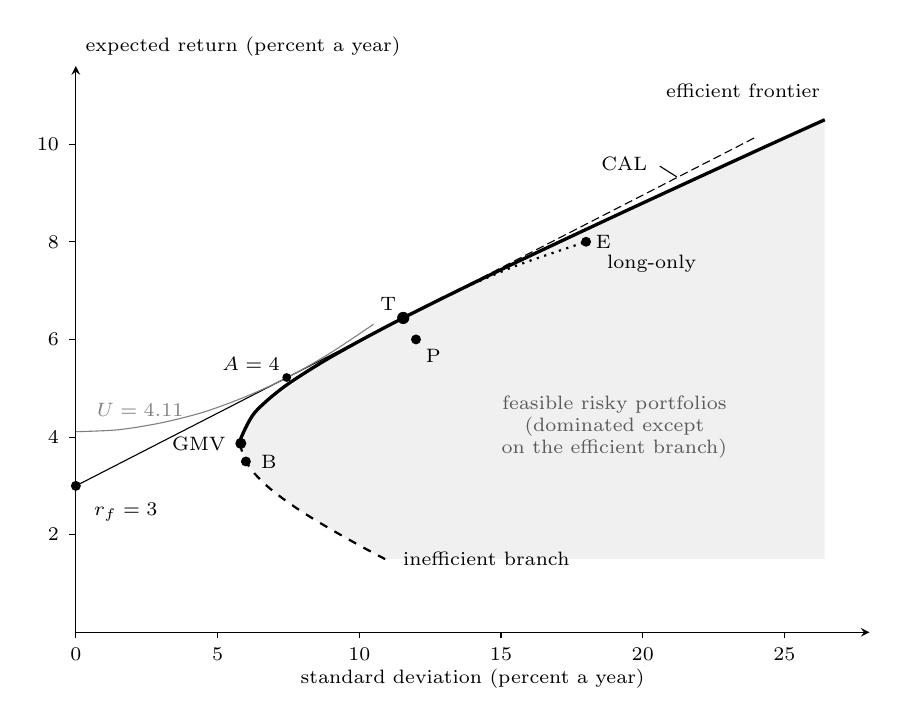
\begin{tikzpicture}[>=stealth, x=0.36cm, y=0.62cm, font=\scriptsize]
  % dominated region: interior of the unconstrained feasible set below the efficient branch (illustrative shading)
  \fill[gray!12] (5.82,3.87) -- (6.31,4.50) -- (8.59,5.50) -- (11.75,6.50) -- (15.25,7.50) -- (18.91,8.50) -- (22.64,9.50) -- (26.42,10.50) -- (26.42,1.50) -- (10.91,1.50) -- (9.33,2.00) -- (7.90,2.50) -- (6.74,3.00) -- (6.00,3.50) -- cycle;
  \node[gray!70!black, align=center] at (19,4.2) {feasible risky portfolios\\(dominated except\\on the efficient branch)};
  \draw[->] (0,0) -- (28,0);
  \node at (14,-0.95) {standard deviation (percent a year)};
  \draw[->] (0,0) -- (0,11.6) node[above right] {expected return (percent a year)};
  \foreach \x in {0,5,10,15,20,25} \draw (\x,0) -- (\x,-0.12) node[below] {\x};
  \foreach \y in {2,4,6,8,10} \draw (0,\y) -- (-0.25,\y) node[left] {\y};
  % efficient
  \draw[very thick] plot[smooth] coordinates {(5.82,3.87) (5.84,4.00) (6.31,4.50) (7.28,5.00) (8.59,5.50) (10.11,6.00) (11.75,6.50) (13.48,7.00) (15.25,7.50) (17.07,8.00) (18.91,8.50) (20.77,9.00) (22.64,9.50) (24.52,10.00) (26.42,10.50)};
  % inefficient
  \draw[thick, dashed] plot[smooth] coordinates {(5.82,3.87) (5.84,3.75) (6.00,3.50) (6.31,3.25) (6.74,3.00) (7.28,2.75) (7.90,2.50) (8.59,2.25) (9.33,2.00) (10.10,1.75) (10.91,1.50)};
  % long-only
  \draw[thick, dotted] plot[smooth] coordinates {(13.48,7.00) (15.49,7.50) (18.00,8.00)};
  % capital allocation line from the risk-free rate through the tangency portfolio, slope 0.2978
  \draw[thin] (0,3) -- (11.55,6.44);
  \draw[thin, dash pattern=on 3pt off 1.5pt] (11.55,6.44) -- (24,10.147);
  % indifference curve of A = 4 through its optimum on the CAL: E = 4.108 + 0.02 s^2
  \draw[thin, gray] plot[smooth] coordinates {(0.00,4.11) (1.50,4.15) (3.00,4.29) (4.50,4.51) (6.00,4.83) (7.50,5.23) (9.00,5.73) (10.50,6.31)};
  \fill (11.55,6.44) circle (2.2pt) node[above left=-1pt] {T};
  \fill (5.82,3.87) circle (2pt) node[left=2pt] {GMV};
  \fill (18,8) circle (1.8pt) node[right] {E};
  \fill (6,3.5) circle (1.8pt) node[right=2pt] {B};
  \fill (12,6) circle (1.8pt) node[below right] {P};
  \fill (0,3) circle (1.8pt);
  \node[anchor=north west] at (0.3,2.85) {$r_f=3$};
  \fill (7.44,5.22) circle (1.6pt) node[above left=-1pt] {$A=4$};
  \node[anchor=east] at (20.5,9.6) {CAL};
  \draw[thin] (20.6,9.55) -- (21.2,9.33);
  \node[anchor=south east] at (26.6,10.75) {efficient frontier};
  \node[anchor=west] at (11.2,1.5) {inefficient branch};
  \node[anchor=west] at (18.4,7.55) {long-only};
  \node[gray, anchor=west] at (0.4,4.55) {$U=4.11$};
\end{tikzpicture}

\end{center}

\qffield{Pitfalls} Calling the lowest-volatility asset the minimum-variance portfolio. Choosing a portfolio on the lower branch. Quoting an unconstrained frontier for an account that cannot short, or a target beyond what its limits allow. Forgetting that the frontier is drawn from estimated inputs, so that an ``efficient'' portfolio is efficient only for those inputs (\hyperref[meth:resampled-efficiency]{resampled efficiency}; DeMiguel et al.\ in \hyperref[mod:mean-variance-portfolio-optimisation]{mean--variance optimisation}). Markowitz plots $V$ against $E$ with $E$ horizontal (p.~82, Fig.~1) and Sharpe puts standard deviation on the vertical axis; most later diagrams, including this one, put risk on the horizontal axis.

\qffield{See also} \hyperref[meth:portfolio-return-moments]{portfolio return moments}; \hyperref[mech:diversification-correlation]{diversification}; \hyperref[meth:capital-allocation-line]{capital allocation line}; \hyperref[mod:mean-variance-portfolio-optimisation]{mean--variance optimisation}.

\end{qfmethod}

\begin{qfmethod}[Adding a risk-free asset: the capital allocation line, the tangency portfolio, separation, the optimal allocation for a given risk aversion, borrowing and leverage assumptions, and the capital market line as an equilibrium special case]\label{meth:capital-allocation-line}
\qffield{Statement} A fraction $x$ in a risk-free security and $1-x$ in a risky portfolio $g$ gives $E(R_p)=xR_f+(1-x)E(R_g)$ and $\sigma(R_p)=(1-x)\sigma(R_g)$ for $x\le1$, so such combinations plot on a straight line from $R_f$ through $g$. Points beyond $g$ represent ``borrowing at the risk-free rate, with the proceeds from the borrowing used to increase investment in portfolio $g$''. Swinging the line up to the tangency portfolio $T$ makes ``all efficient portfolios \dots\ combinations of the risk-free asset (either risk-free borrowing or lending) and a single risky tangency portfolio'', Tobin's separation theorem \citep[\emph{JEP} 18(3), 2004, pp.~27--28 and n.~2]{capm-theory-evidence-2004}.

Sharpe derives the same line and adds that when the borrowing rate equals the lending rate, choice divides into selecting the risky combination and then borrowing or lending to reach the investor's preferred point \citep[\emph{Journal of Finance} 19(3), 1964, pp.~432--433]{capital-asset-prices-1964}.

\qffield{Notation} Write $y=1-x$ for the share in the risky portfolio. A \emph{capital allocation line} (CAL) is
\[ E(r_p)=r_f+\frac{E(r_g)-r_f}{\sigma_g}\,\sigma_p, \]
whose slope is the Sharpe ratio of $g$. The tangency portfolio maximises that slope. With a budget constraint only, it is $w_T=\Sigma^{-1}(\mu-r_f\mathbf 1)/\mathbf 1^\top\Sigma^{-1}(\mu-r_f\mathbf 1)$ (Interpretation). Maximising $U=r_f+y[E(r_T)-r_f]-\tfrac12Ay^2\sigma_T^2$ gives
\[ y^\ast=\frac{E(r_T)-r_f}{A\,\sigma_T^2}; \]
$y^\ast<1$ means lending, $y^\ast>1$ borrowing (\hyperref[def:risk-aversion-utility]{risk aversion and utility}).

\qffield{Conditions} \emph{Tangency formula.} It needs $\Sigma$ positive definite and $r_f$ below the GMV mean $B/A$, so that $\mathbf 1^\top\Sigma^{-1}(\mu-r_f\mathbf 1)=B-r_fA>0$. Otherwise the normalised vector lies on the lower branch and no efficient tangency exists. Short-sale limits replace the formula by a constrained maximisation of the Sharpe ratio (Interpretation).

\emph{Risk-free asset.} The asset must be riskless over the investor's horizon and in the investor's currency, which a nominal Treasury bill matching the horizon approximates in nominal terms only. Borrowing at the lending rate in unlimited amounts is a strong assumption. Fama and French describe unrestricted risk-free borrowing and lending as ``an unrealistic assumption'' (p.~29), and margin rules, financing spreads and leverage limits bound $y$ in practice. Sharpe argues that the assumption is less onerous than it seems: an investor who cannot borrow but wants a point below the tangency still chooses it and lends, and with borrowing limited only the most risk-tolerant investors choose otherwise (p.~433).

With a borrowing rate above the lending rate the efficient set has three parts. The lending line runs to its tangency; a stretch of the risky frontier follows; the borrowing line starts at a second, riskier tangency (Interpretation).

\emph{CAL against CML.} Any line from $r_f$ through a risky portfolio is a CAL, and the best one depends on the investor's own estimates. The \emph{capital market line} (CML) is the CAL through the market portfolio. Identifying the two needs equilibrium assumptions: a common pure rate for borrowing and lending and homogeneous expectations, which Sharpe calls ``highly restrictive and undoubtedly unrealistic'' (pp.~433--434). Prices then adjust until every asset enters a combination on the CML (p.~435).

Fama and French state the same assumptions as complete agreement on the true joint distribution of returns and borrowing and lending at a common risk-free rate (p.~26). With them ``all investors see the same opportunity set'', hold the same tangency portfolio, and market clearing makes it ``the value-weight market portfolio of risky assets'' (p.~28). In Black's version short sales replace the risk-free asset (pp.~29--30). Without these assumptions the market portfolio need not be any investor's tangency portfolio, and its proxies are discussed in \hyperref[mod:capm-sml]{CAPM}.

\qffield{Practice} Example, original: the three funds of this section with $r_f=3$ percent. The GMV mean of 3.87 percent exceeds $r_f$, so the tangency exists: $w_T=(0.437,0.175,0.388)$, with $E(r_T)=6.44$ and $\sigma_T=11.55$ percent, and a Sharpe ratio of 0.298. A numerical maximisation of the Sharpe ratio returns the same weights, and the CALs through the GMV, the 7 percent frontier portfolio and a 60/20/20 mix are flatter.

\begin{center}\small
\begin{tabular}{@{}rrrrr@{}}
\toprule
$A$ & $y^\ast$ & Position & $E(r_p)$ & $\sigma_p$ \\
\midrule
2 & 1.289 & borrow 28.9 percent of wealth & 7.43 & 14.89 \\
4 & 0.645 & lend 35.5 percent & 5.22 & 7.44 \\
8 & 0.322 & lend 67.8 percent & 4.11 & 3.72 \\
\bottomrule
\end{tabular}
\end{center}

All three investors hold the same risky mix and differ only in how much of it they hold. A grid search over $y$ confirms each optimum. The $A=4$ point and its indifference curve, with $U=4.11$ percent, are drawn in the \hyperref[meth:efficient-frontier]{efficient frontier} figure.

\emph{Borrowing at a higher rate.} Suppose lending is at 3 percent but borrowing costs 3.5 percent, still below the GMV mean. The borrowing tangency is $(0.951,-0.787,0.836)$, with mean 9.87 and standard deviation 24.03 percent. The $A=2$ investor would borrow on the lending line ($y^\ast=1.29$) but would lend on the borrowing line ($y=0.55$). That investor therefore holds a frontier portfolio with no riskless position: mean 7.18, standard deviation 14.11 percent and $U=5.19$ percent, which here includes a small short in B. A 5 percent borrowing rate would exceed the GMV mean, and the tangency formula would return a lower-branch portfolio with mean 1.88 percent.

\qffield{Pitfalls} Placing individual assets on the CML: only efficient portfolios lie on it, and single assets lie below it (\hyperref[mech:systematic-risk-pricing]{systematic risk}). Treating leverage as free or unlimited. Ranking portfolios by the Sharpe ratio for an investor who cannot borrow and wants more return than the tangency offers. Applying the tangency formula when $r_f$ is above the GMV mean. Calling a CAL built on one investor's estimates the CML.

\qffield{See also} \hyperref[meth:efficient-frontier]{efficient frontier}; \hyperref[def:risk-aversion-utility]{risk aversion and utility}; \hyperref[mod:capm-sml]{CAPM and the security market line}; \hyperref[mod:mean-variance-portfolio-optimisation]{mean--variance optimisation} (maximum-Sharpe objective).

\end{qfmethod}
